\documentclass[11pt,letterpaper]{article}
\usepackage[lmargin=1in,rmargin=1in,tmargin=1in,bmargin=1in]{geometry}

% -------------------
% Packages
% -------------------
\usepackage{
	amsmath,			% Math Environments
	amssymb,			% Extended Symbols
	enumerate,		% Enumerate Environments
	graphicx,			% Include Images    
	lastpage,			% Reference Lastpage
	multicol,			% Use Multi-columns
	multirow,			% Use Multi-rows
	siunitx
}

\graphicspath{{./images/}}

\usepackage{wrapfig}

% -------------------
% Font
% -------------------
\usepackage[T1]{fontenc}
\usepackage{charter}    


% -------------------
% Heading Commands
% -------------------
\newcommand{\class}{Mu Alpha Theta}
\newcommand{\term}{2022-2023}
\newcommand{\head}[3]{%
\thispagestyle{empty}
\vspace*{-0.5in}
\noindent\begin{tabular*}{\textwidth}{l @{\extracolsep{\fill}} r @{\extracolsep{6pt}} l}
	\textbf{#1} & \textbf{Name:} & \makebox[5.75cm]{\hrulefill} \\
	\textbf{#2} & & \\
	\textbf{\class:\; \term} & & \\
\end{tabular*} \\
\rule[2ex]{\textwidth}{2pt} %
}


% -------------------
% Commands
% -------------------
\newcommand{\prob}{\noindent\textbf{Problem. }}
\newcounter{problem}
\newcommand{\problem}{
	\stepcounter{problem}%
	\noindent \textbf{Problem \theproblem. }%
}
\newcommand{\pointproblem}[1]{
	\stepcounter{problem}%
	\noindent \textbf{Problem \theproblem.} (#1 points)\,%
}
\newcommand{\pspace}{\par\vspace{\baselineskip}}
\newcommand{\ds}{\displaystyle}


% -------------------
% Header & Footer
% -------------------
\usepackage{fancyhdr}

\fancypagestyle{pages}{
	%Headers
	\fancyhead[L]{}
	\fancyhead[C]{}
	\fancyhead[R]{}
\renewcommand{\headrulewidth}{0pt}
	%Footers
	\fancyfoot[L]{}
	\fancyfoot[C]{}
	\fancyfoot[R]{}
\renewcommand{\footrulewidth}{0.0pt}
}
\headheight=0pt
\footskip=14pt

\pagestyle{pages}


% -------------------
% Content
% -------------------

\begin{document}
\head{Worksheet \#3}{Date:}
\centering

% Question 1: https://artofproblemsolving.com/wiki/index.php/2006_AMC_10B_Problems/Problem_8
\begin{minipage}{\textwidth}
     \problem

     \begin{wrapfigure}[11]{r}{0.6\textwidth}
          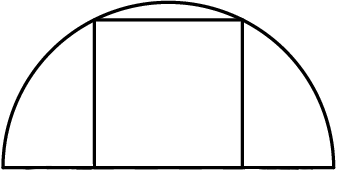
\includegraphics[width = 6.5cm]{images/AMC-10-2006-P8.png}
     \end{wrapfigure}
     \noindent A square of area $40$ is inscribed in a semicircle as shown. What is the area of the semicircle?
\end{minipage}
\vspace{7cm}

% Question 2: https://artofproblemsolving.com/wiki/index.php/2008_AMC_12A_Problems/Problem_22
\begin{minipage}{\textwidth}
     \problem
     
     

     \noindent This a multiplicative magic square. That is, the product of the numbers in each row, column, and diagonal is the same. If all the entries are positive integers, what is the sum of the possible values of $g$?
     
     \vspace{1cm}
     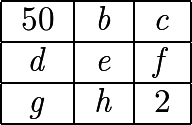
\includegraphics[width = 3cm]{images/AMC-12-2004-P22.png}
     
\end{minipage}

\vspace{6cm}
% Question 3: https://artofproblemsolving.com/wiki/index.php/2009_AMC_10A_Problems/Problem_10
\begin{minipage}{\textwidth}
     \problem

     \noindent Triangle $ABC$ has a right angle at $B$. Point $D$ is the foot of the altitude from $B$, $AD=3$, and $DC=4$. What is the area of $\triangle ABC$?
     \vspace{1cm}

     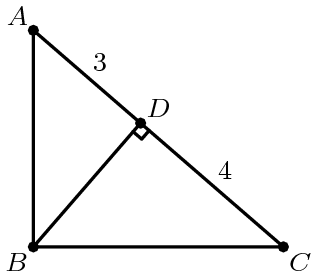
\includegraphics[height = 4cm]{images/AMC-10-2009-P10.png}
     
\end{minipage}
\vspace{2cm}

% Question 4: https://artofproblemsolving.com/wiki/index.php/2008_AMC_12A_Problems/Problem_11
\begin{minipage}{\textwidth}
     \problem

     \noindent Three cubes are each formed from the pattern shown. They are then stacked on a table one on top of another so that the $13$ visible numbers have the greatest possible sum. What is that sum?

     \vspace{1cm}
     
     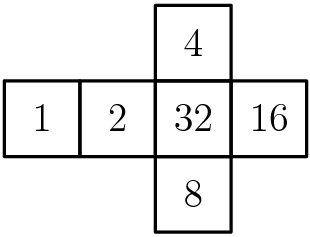
\includegraphics[width=0.25\textwidth]{images/AMC-12-2008-P11.png}

\end{minipage}
\vspace{2cm}


% Question 5: https://artofproblemsolving.com/wiki/index.php/2007_AMC_10B_Problems/Problem_19
\begin{minipage}{\textwidth}
     \problem

     \noindent The wheel shown is spun twice, and the randomly determined numbers opposite the pointer are recorded. The first number is divided by $4,$ and the second number is divided by $5.$ The first remainder designates a column, and the second remainder designates a row on the checkerboard shown. What is the probability that the pair of numbers designates a shaded square?

     \vspace{1cm}

     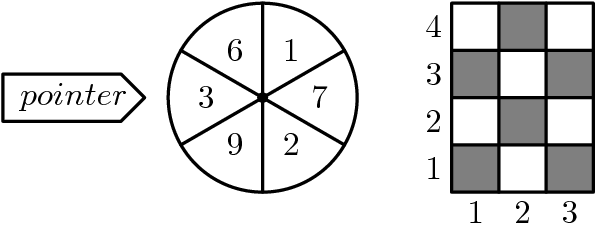
\includegraphics[width = 8cm]{images/AMC-10-2007-P19.png}   

\end{minipage}
\vspace{2cm}


\end{document}